\documentclass[a4paper]{article}
%\usepackage{fourier-otf}
\usepackage[utf8]{inputenc}
\usepackage{graphicx}
\usepackage{amsmath}
\usepackage{amsfonts}
\usepackage{float}
\usepackage{biblatex}
\addbibresource{bibliography.bib}
\usepackage{listings}
%\usepackage[square,sort,comma,numbers]{natbib}
\newtheorem{theorem}{Theorem}[section]
\usepackage{color}
\usepackage{makeidx}
\usepackage{titlepic}
\definecolor{mygreen}{rgb}{0,0.6,0}
\definecolor{mygray}{rgb}{0.5,0.5,0.5}
\definecolor{mymauve}{rgb}{0.58,0,0.82}
\lstset{ %
	backgroundcolor=\color{white},   % choose the background color
	basicstyle=\footnotesize,        % size of fonts used for the code
	breaklines=true,                 % automatic line breaking only at whitespace
	captionpos=b,                    % sets the caption-position to bottom
	commentstyle=\color{mygreen},    % comment style
	escapeinside={\%*}{*)},          % if you want to add LaTeX within your code
	keywordstyle=\color{blue},       % keyword style
	stringstyle=\color{mymauve},     % string literal style
}
\usepackage{hyperref}
\hypersetup{
  colorlinks   = true,    % Colours links instead of ugly boxes
  urlcolor     = black,    % Colour for external hyperlinks
  linkcolor    = black,    % Colour of internal links
  citecolor    = black      % Colour of citations
}
\title{First chapter}

\author{F.Bernardi}







\begin{document}
		\maketitle
		
		\begin{minipage}{\linewidth}
			\centering
			\begin{minipage}{0.45\linewidth}
				\begin{figure}[H]
					
\includegraphics[width=\linewidth]{Logo_IIT.png}
					
				\end{figure}
			\end{minipage}
			\hspace{0.05\linewidth}
			\begin{minipage}{0.45\linewidth}
				\begin{figure}[H]
					
\includegraphics[width=\linewidth]{Logo_Politecnico_Milano.jpg}
					
				\end{figure}
			\end{minipage}
		\end{minipage}
	
	\clearpage
	
	\tableofcontents
	
	
	
	\clearpage
	
	\section{Neurobiology of behaviour}
	
	
	In this first chapter, the biological and experimental foundations of this work will be presented. After a brief review of the main notions of neurobiology, such as the structure of a neuron, the propagation of an action potential in neuronal circuits and the intracellular calcium dynamics, there will be a closer focus on the areas of the brain interested in the following discussions.\\
	Next, the experimental setup for such studies is presented, through the description of the behavioral tasks performed on mice and the experimental techniques for calcium imaging, from which it will be possible to extract the data analyzed in Chapter 2.\\
	Finally, a  quite modern and extremely relevant topic for this work is introduced: the synchronization between neural signals.
	
	\subsection{Neuronal circuits to describe behaviour}
	
	\begin{figure}[H]
		\begin{center}
			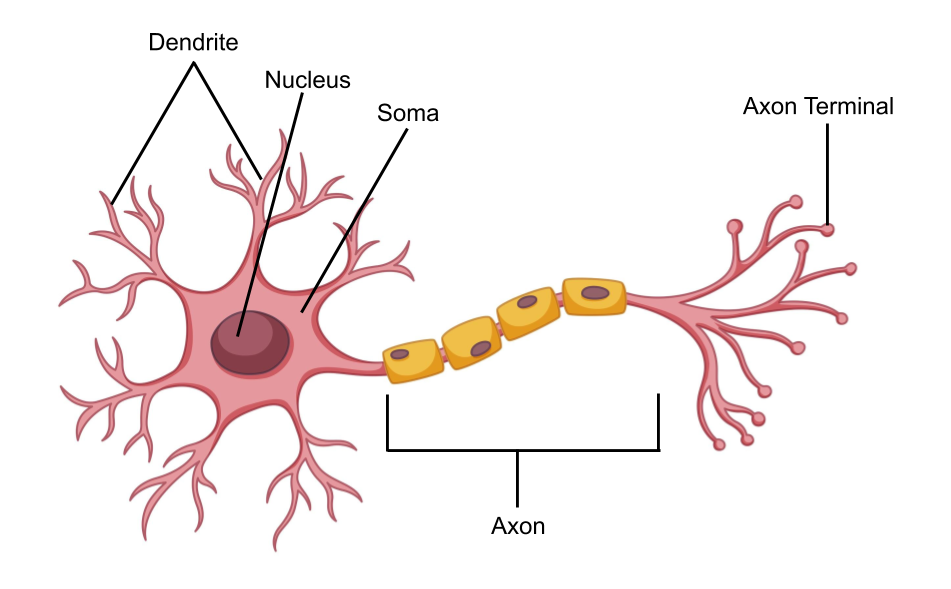
\includegraphics[scale=.25]{neuron.png} 
		\end{center} 
		\caption{\textit{Schematic representation of a neuron}}
		
	\end{figure}
	
	The importance of the brain in mammals is by today extremely evident: this vital organ allows us to think,  to capture the stimuli from the environment and elaborate them, enriching our memory and  our learning. It is the control center of our movements and our actions, it allows us to speak, to understand other individuals and elaborate responses. Most importantly for this work, however, the brain, from its basic cellular units, can explain our behaviour and our emotions. \\
	
	The brain itself is part of the \textbf{nervous system (NS)}, and its most important cell is the \textbf{neuron}: it is the basic unit needed for the transmission of the electric signal, both within the same area and between different areas of the organism, allowing the NS to collect information and to react to stimuli, elaborating decisions based on them. \\
	The neuron is composed of a central body called \textit{soma}, where all the cellular functionalities happen, of the \textit{dendrites}, cellular extensions which collect stimuli from near areas, and of the \textit{axon}, the biological cable connecting one neuron to another, in order to propagate information. 
	The second type of cells present in the NS are the \textbf{glial cells} (like astrocytes) , which perform functions of protection, sustainment and nutrition for the neurons. Although they won't be treated much in this work, their contribution should not be neglected, as it has been shown to be relevant in many important processes of the nervous system [Semyanov, Henneberger 2020]. \\
	
		
	
	Neurons are \textbf{excitable} and \textbf{conductive}, i.e. they can generate an electrical impulse and transmit it to other neurons, forming neuronal microcircuits, often associated with a specific area and/or task of the brain. \\
	Inside every neuron, in the cytoplasm, there is a coexistence of different ionic species (mostly $Na^+, Cl^-, K^+, Ca^{2+}$) which, in equilibrium conditions, assume a certain concentration, determining itself a difference between the potential assumed inside and outside the cell: we call this quantity the \textbf{membrane potential} of the cell (indeed it is the potential formed across the cell's membrane).  In reaction to an external stimulus, the ionic concentrations change rapidly their values, provoking a heavy change in the membrane potential: here the excitation of a neuron happens, as well as the formation of an \textbf{action potential}, which will propagate to other neurons across the axon. 
\begin{figure}[H]
	\begin{minipage}{\linewidth}
		\centering
		\begin{minipage}{0.45\linewidth}
			\begin{figure}[H]
				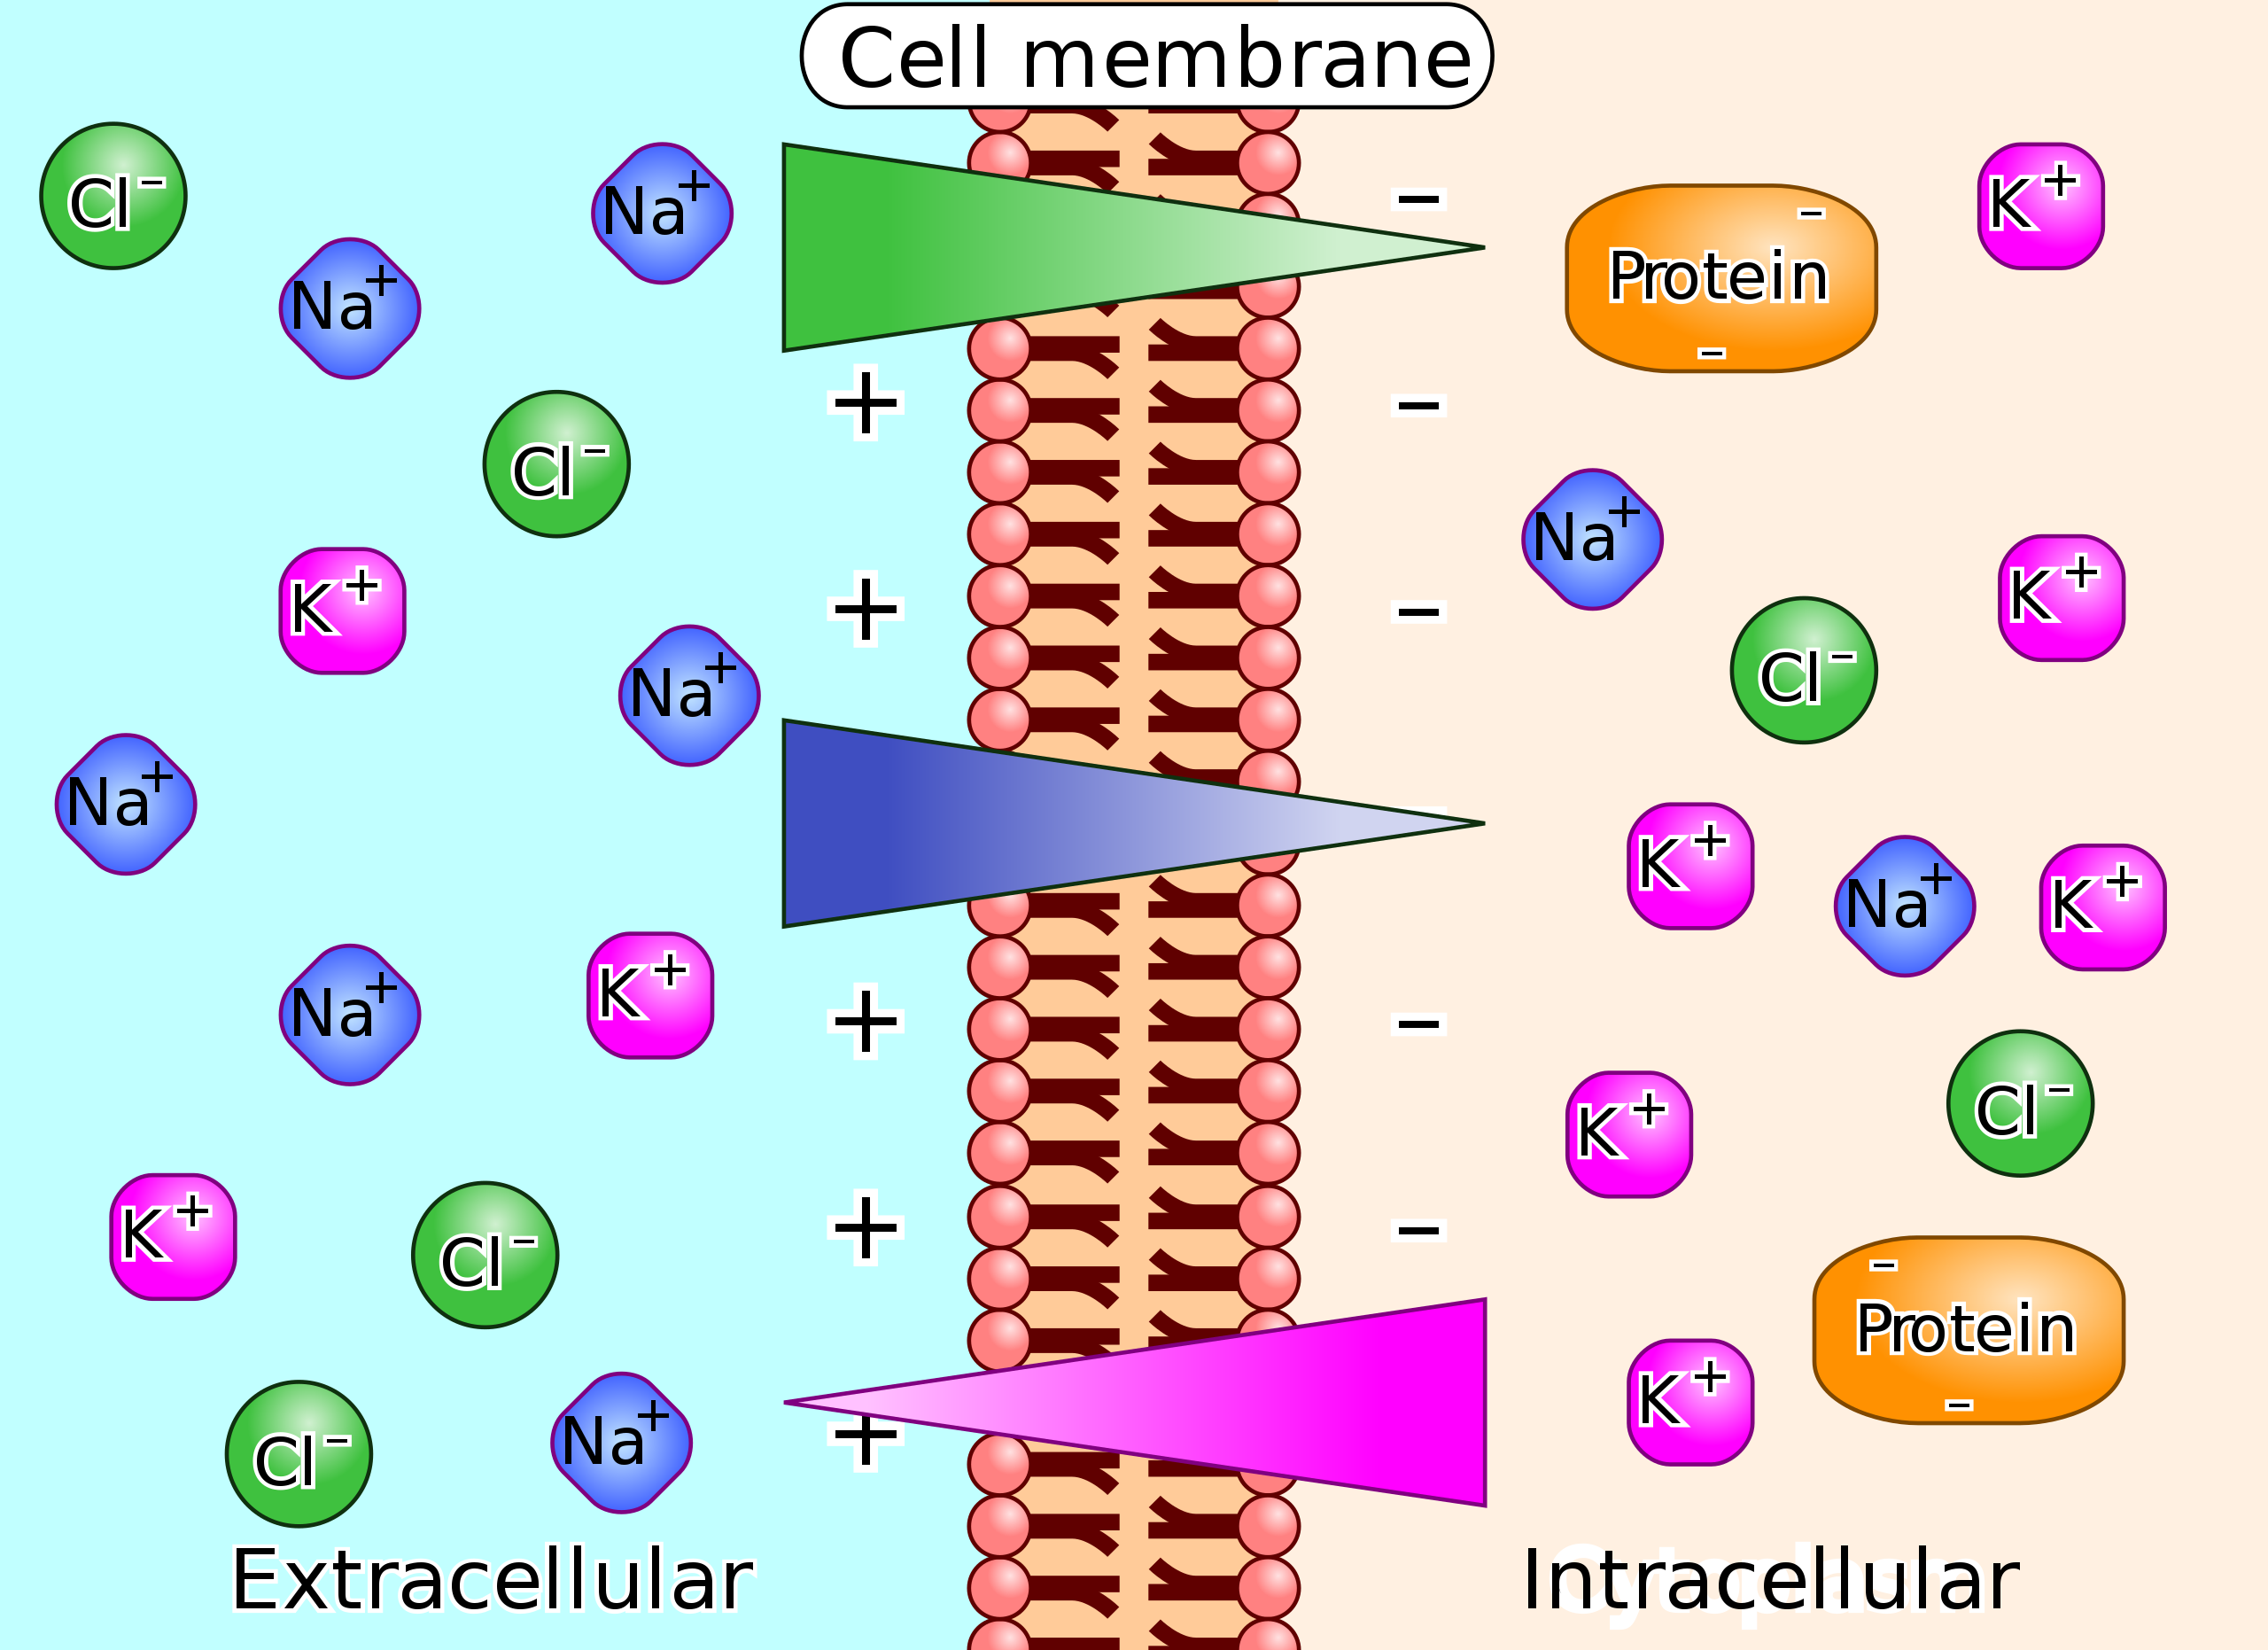
\includegraphics[width=\linewidth]{AP1.png}
				
			\end{figure}
		\end{minipage}
		\hspace{0.05\linewidth}
		\begin{minipage}{0.45\linewidth}
			\begin{figure}[H]
				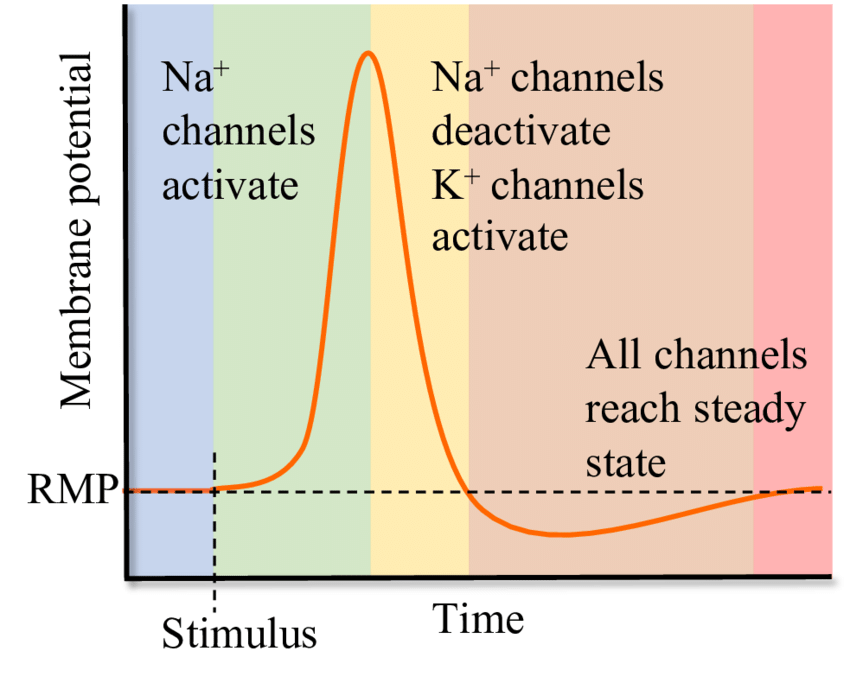
\includegraphics[width=\linewidth]{AP2.png}
				
			\end{figure}
		\end{minipage}
		
	\end{minipage}
\caption{\textit{Left: schematic representation of ionic species inside and outside the cellular membrane. Such species are allowed to pass through the membrane only in specific circumstances through adhibited ionic gates \\
Right: example of action potential formation in reaction to a stimulus}}
\end{figure}

At the end of the axon, the link between a neuron and its neighbour, and the relative passage of the electrical impulse, happens thanks to a chemical \textbf{synapse}, a particular structure located in the terminal of the axon. Here, special molecules called \textit{neurotransmitters} are syntethized, and the arrival of an action potential allows such molecules to travel towards the \textit{intersynaptic space}, where they can bind to receptors located in the post-synaptic cell. The response of the post-synaptic cell, then, can be either excitatory or inhibitory, based on whether the impulse is preserved in the circuit or supressed.\\
The synapses (and thus their correspondent neuron) can be classified in four main groups, depending on the type of neurotransmitter which they release:  glutamatergic, GABAergic, cholinergic,  adrenergic. The most relevant for this work will be the GABAergic one, consisting of inhibitory neurotransmitters which reduce the excitability of the neurons.
\begin{figure}[H]
	\begin{center}
		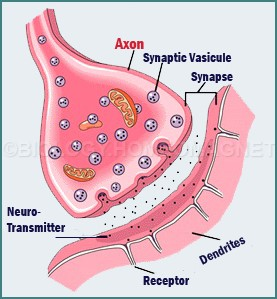
\includegraphics[scale=1.6]{synapse.jpg} 
	\end{center} 
	\caption{\textit{Schematic representation of a chemical synapse}}
	
\end{figure}



In neurobiology, the conditions under which a neuron can be considered \textbf{active} are not unique and matter of debate; in general, however, when talking about neural activity, the literature usually means either the already discussed electrical activity, either the \textbf{calcium activity}. The intracellular dynamic of this particular element, in ionic form of $Ca^{2+}$, is known to be essential for the main cellular processes, and it is strictly related to the formation of an action potential and subsequent propagation of the electrical impulse.\\
 Indeed, we can usually observe  \textit{strong instabilities} in the intracellular calcium concentration values, which often show fast oscillations and changes, through the formation of sudden peaks: we will define the neuron as \textit{active} in correspondence to these peaks.

\begin{figure}[H]
	\begin{center}
		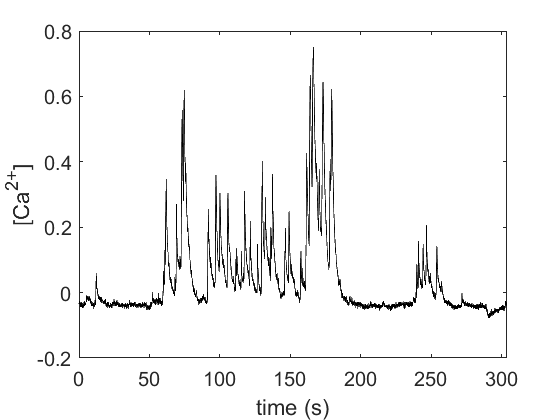
\includegraphics[scale=.50]{Ca_conc.png} 
	\end{center} 
	\caption{\textit{Example of $Ca^{2+}$ concentration recorded in a neuron, as function of time}}
		
	\end{figure}
	
	Once defined the meaning of neuronal activity, we can ask ourselves whether this activity could be related to aspects like behaviour, emotion, body language, mood: in other words, to investigate whether there is a connection between the activation of some specific neurons, and what animals feel or do.\\
	This topic has fascinated neuroscientists for decades, and from what it has been discovered so far, it seems evident that \textbf{different areas of the brain are responsible for different emotions, feelings or behaviours} (although these distinctions may not always be that marked, unique and easy to detect).

	
	The neurobiology experiments on which this work relies on refer mainly to some particular areas of the brain, which previous studies found to be strictly connected to emotional and behavioral processes [Etkin et al. 2011]:
	\begin{itemize}
		
		\item \textbf{Medial prefrontal cortex (mPFC)}:  part of the frontal cortex, the area of the brain located in the frontal lobe. This area is implicated in cognition processes like emotional or social, but strong connections with decision making have been found as well [Carlen 2017]
		
		\item \textbf{Anterior Cingulate Cortex (ACC)}: part of the cingulate cortex and situated in proximity of the mPFC,  of which the ACC shares a lot of functionalities. Indeed, experimental evidence of the connection between this area of the brain and emotions have been found [Zheng 2020]. This area seems also to be implicated in social aspects like morality or empathy [Carillo 2019], as reaction to interactions with another individual
		
		\item \textbf{Amygdala}: nuclear complex located in the medial part of the temporal lobe. It is responsible for the elaboration of the emotions, it collects stimuli from the thalamus and elaborate responses: in other words, it's a sort of emotional thermometer of the body and the decision maker for adequate responses [ARTICOLO?]
	\end{itemize}


	
	\begin{figure}[H]
		\begin{center}
			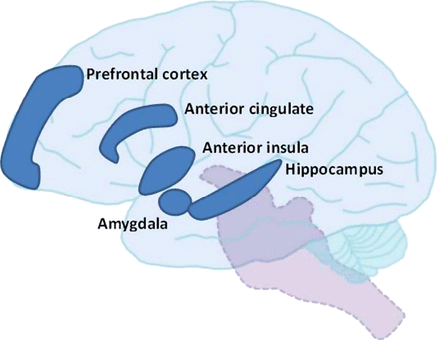
\includegraphics[scale=.55]{brain.png} 
		\end{center} 
		\caption{\textit{Main areas of the brain involved in behaviour and emotion recognition}}
		
	\end{figure}

\newpage

\subsection{In vivo studies on mice}

According to the \textit{Foundation of Biomedical Research (FMR)}, approximately $95\% $ of all lab animals are mice or rats, as it is in the case of this current work. Although very often the final goal of the research is an application useful for humans, the reasons why mice are the first choice for experiments are numerous: first of all, mice are mammals quite similar to humans when it concerns genetics, at the point that scientists have been able to reproduce genes in mice similar to the ones implied in human diseases ("\textit{transgenic mice}" [Harari,Abramovich 2014]); rodents, indeed, are also easy to manipulate from a genetic point of view. Another reason is surely the convenience: mice are small, easy to control, quite cheap to buy and usually docile. Finally, being the most used animal in research, the largest information and literature which can be found is about them, their anatomy, their typical behaviours, and by today large populations of rodents have been created and used exclusively for experimental purposes, being almost all identical between them and therefore setting a uniform standard for study and validation of results. \\
Through a  \textbf{behavioral task}, one or more mice are put in a particular situation created to study their reactions, such as a shown behaviour or movement, and, in this context, the goal is to find a relationship with their correspondent neural activity. Therefore, the overall experiment consists in the following steps:
\begin{enumerate}
	\item Preparation of the arena and equipment for the task 
	\item Preparation of the mice for the experiment, both in terms of behavioral conditioning, and for neural activity measurments
	\item Performance of the test with simultaneous recordings of  aspects of interest such as behaviour or neuronal activity
	\item Pre-processing and analysis of the collected data
\end{enumerate}

\begin{figure}
	\begin{center}
		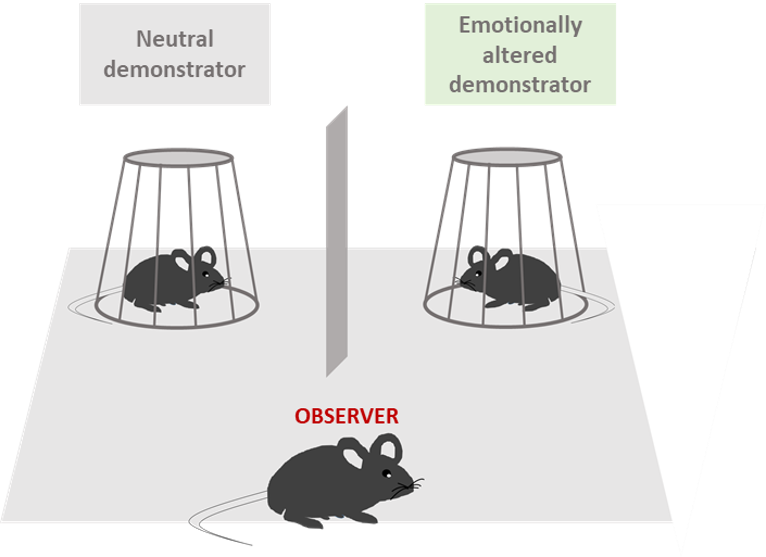
\includegraphics[scale=.60]{mice_task.png} 
	\end{center} 
	\caption{\textit{Basic setting of the emotion discrimination task: one mouse (the \textit{observer}) is free to move in the arena, while the others two (the \textit{demonstrators}) remain inside a cage. One of the demonstrators has a neutral affective state, the other an altered affective state}}
	
\end{figure}
In this work, the behavioural task which has been studied is a particular realization of the \textbf{emotion discrimination task}. The first step of these types of tasks, performed in this way several times in the past, sees the presence of three mice: one, called the \textbf{observer}, is a mouse free to move in an arena, while the others, the \textbf{demonstrators}, remain in a cage. In the phase preceding the test, the \textit{habituation phase}, one of the two demonstrators is \textit{emotionally altered}: namely, it is subjected to specific conditions and procedures which provoke an alteration of his affective state. This alteration could be either negative (usually stress condition following a period of water deprivation) or positive (usually relief condition, consisting in water \textit{ad libitum} following water deprivation). The other demonstrator, such as the observer, is instead in a \textit{neutral} state.\\

Previous works on this setup [Scheggia-Managò] were performed using both positive and negative affected demonstrators. The cellular target consisted in a specific subpopulation of neurons, which is thought to be involved in processes like \textit{affective state discrimination}: the SOM+ interneurons in the medial prefrontal cortex.\\
These neurons, expressing the \textbf{somatostatin} neurotransmitter, form a small group compared to others like \textit{pyramidal neurons} or \textit{parvalbumin neurons}, but unlike these former ones, they seem to be directly implicated in the affective state discrimination of a conspecific. The data analysis on the task showed some remarkable results:

 \begin{itemize}
 	
 	\item The time spent by the observer near the altered demonstrator was significantly higher than the one spent near the neutral one, such as the duration of the moments when reciprocal sniffing between two close mice happened
 	
 	\item This  discrimination appears to be stronger in the first period of the test
 	
 	\item The discrimination is directly connected to the presence of a mouse in an altered state (both negative and positive), since from the repetition of the task using only two neutral demonstrators no significant differences emerged
 	
 	\item It has been shown that the main sense responsible for the discrimination is olfaction, but to achieve the same results of the test, a combination of all senses is needed
 	
 	\item The neural activity of the observer (both in terms of electrical impulse and  calcium peaks) showed stronger values during the interactions with the altered mouse rather than the neutral one
 	
 	\item  If a mechanism of \textit{optical inhibition} of SOM+ cells [REFERENCE?] is performed before the test, the discrimination disappears, namely no relevant differences between time spent, sniffing and neural activity have been observed with the altered demonstrator rather than with the neutral one
 	
 	\item All the previous considerations do not apply to other neuronal categories like pyramidal or parvalbumin interneurons
 	 
 \end{itemize}
 
 Overall, these results seem to show a \textbf{key role of the somatostatin interneurons in affective state discrimination}.

	\begin{figure}
	\begin{center}
		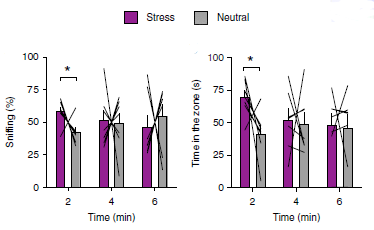
\includegraphics[scale=.99]{scheggia.png} 
	\end{center} 
	\caption{\textit{Recording of sniffing times (left) and proximity times (right) between observer mouse and stressed demonstrator}}
	
\end{figure}


Other examples of emotion discrimination in mice related to SOM+ interneurons can be found in [Mariotti et al 2018], with a focus on their effect on cortical astrocytes: the main result shown in the study consist in a \textbf{crucial role of somatostatin} in the stimulation of responses by astrocytes.\\
As a first result, it has been shown that the stimulation of SOM+ interneurons (via 10-pulses light stimulation of GECIs), increases the $Ca^{2+}$ response from astrocytes. Also in this case, a comparison with PV+ (parvalbumin) interneurons show the \textit{critical sensitivity of astrocytes only to SOM+ interneurons, but not PV+}. Overall, this study reveals that a sustained activity in the SOM+ interneuron circuits is complemented by
a sustained activity in the astrocytic network, as confirmation of the importance of astrocytes and their link to inhibitory neuronal circuits. 
\\

Somatostatin interneurons are not the only neuropeptide that has been shown to be deeply linked to emotion discrimination. For example, in [Ferretti-Maltese 2018], the in vivo task on mice targets the \textbf{oxytocin (OXT)} neurotransmitter, studying its release in the central amygdala. The behavioral task of this study has a similar structure to [Scheggia-Manago], in which neutral and altered demonstrators were contraposed to an observer mouse. Also in this case, evidence of  discrimination caused by the altered mouse (through, for example, an increased sniffing activity) has been shown, such as the importance of olfactory clues in the process of such discrimination.\\
The reduction of the OXT levels in the central amygdala resulted in the \textit{abolishment} of emotion discrimination, while a new increase of such levels resulted in the rescue of the former conditions, remarking the central role of the OXT neuropeptide in the emotion discrimination.
\\

Targeting a specific neuronal subpopulation, the hope is to always find  more evidence on its link with  properly shown tendencies, emotions or behaviors that are common to known diseases. In the case of the discussed task targeting SOM+ interneurons in the mPFC, for example, the observed effects in the abolition of discrimination, through photoinhibition of such neurons, could be similar to the ones observed in neurodegenerative disorders such as autism spectrum disorders (ASDs) or schizophrenia. Therefore, this approach aims to investigate the causes of a specific issue at a basic and detailed level such the one of single neuron precision, with the ultimate goal of acting on such level to perform a change on the macroscopic effects.\\
In order to do so, the paradigm of the task has to be defined in a way that it allows a collection of unbiased results, but an adequate way to perform an imaging of the neuronal activity of interest is necessary as well (and described in the following sections). As final step, a proper data analysis on those results has to be performed (chapter 2).


\subsection{Calcium imaging through Inscopix}



\begin{figure}[H]
	\begin{center}
		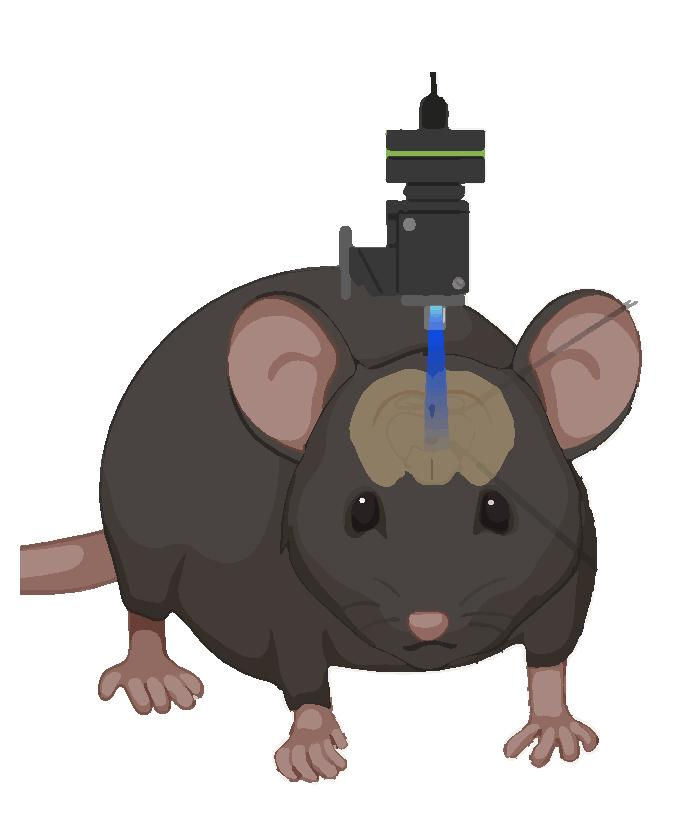
\includegraphics[scale=.35]{Inscopix.jpg} 
	\end{center} 
	\caption{\textit{The Inscopix miniscope}}
	
\end{figure}


In this section, a powerful tool for single neuron calcium imaging will be presented. The Inscopix company [https://www.inscopix.com/] provides tools and software to extract calcium tracks as one photon measurements from in vivo experiments on mice.\\
To measure the intracellular $Ca^{2+}$ concentration in a single mouse during a behavioral task, the first step is the performance of a surgery on the mouse to implant a miniscope in the \textit{region of interest (ROI)} of the brain to be investigated. On the same mouse, \textbf{genetically encoded calcium indicators (GECI)}, such as the \textbf{GCaMP} protein, are adopted. These types of proteins, when bound to $Ca^{2+}$, emit a fluorescent light, which intensity will be captured by the miniscope. At the end of the test, the miniscope will be able to give back a video of the ROI, in which the evolution of the fluorescence through time can be appreciated  in the neurons. In this way, it is possible to obtain a representation of the intracellular calcium oscillations behaviour during the whole task. This information will be combined with behavioral or positional data of the mice in the arena, making it possible to start a data analysis and look for correlations between behaviour and neural activity.\\
In order to have the data ready to be analyzed, however, the Inscopix software manages also the pre-processing part, which goes through the following steps:

\begin{figure}[H]
	\begin{center}
		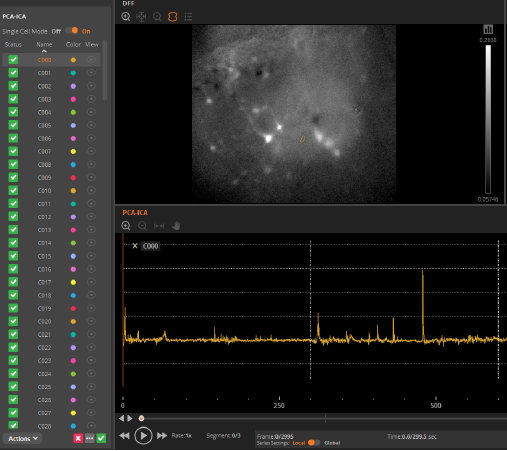
\includegraphics[scale=.70]{Inscopix2.png} 
	\end{center} 
	\caption{\textit{Example of pre-processing work through Inscopix software. We can appreciate: the list of detected neurons (left), a segment of the video in the ROI (top-right) and an example of the calcium track recorded in a single neuron through time (bottom-right)}}
	
\end{figure}

\begin{enumerate}
	
	\item If needed, more videos recorded from the test are combined, in order to obtain a single final video of the ROI through time
	
	\item \textbf{Spatial and temporal downsampling} are performed, selecting the appropriate scale factors of space and time which allow to capture all the important intels
	
	\item \textbf{Spatial filtering} of the image: it removes low and high frequencies with a bandpass filtering. The filter has the form
	
	$$ M_f^{band} = GB(M_f,\sigma_{high}) - GB(M_f,\sigma_{low})$$
	
	Where $M_f$  represents the frame $f$ of movie $M$, $GB$ is the \textit{Gaussian Blur} function, and the standard deviations $ \sigma_i = \frac{2 ln(2)}{2 \pi \lambda_i}$ are computed from the cut-off values $ \lambda_{high}$ and $ \lambda_{low}$
	
	\item \textbf{Motion correction}: it accounts for the motions between different frames of the videos, applying a correction to let every pixel staying at the same place in different frames
	
	\item \textbf{Pixel normalization}: each pixel of a frame represents a different luminosity, caused by the fluorescence in reaction to the GCaMP. After the preprocessing, the value of the fluorescence (which estimates the calcium concentration) is expressed as 
	$$\frac{\Delta F }{F} = \frac{F(x,y,t) - F_b}{F_b}$$
	where $F(x,y,t)$ represents the measured fluorescence in the point $(x,y)$ at time $t$, while $F_b$ is a baseline fluorescence value (usually the mean value of the movie, in some cases the minimum). After this step, the returned value for every pixel is an adimensional relative value of fluorescence
	
	\item The \textbf{PCA-ICA algorithm} attempts to recognize the neurons of the ROI in the movie. Based on given information such as average cell's diameter, a principal component analysis (PCA) is performed, followed by an independent component analysis (ICA), until convergence. In particular, the frames of the movie, represented as matrices, are rasterized into 1D vectors and they are normalized on mean and standard deviation. At this point, a principal component analysis is performed, in order to reduce dimensionality. Every frame is then approximated by a weighted sum of the principal trace components. Finally, an ICA algorithm is launched. At the end of this process, every neuron will be identified, labeled, and gifted with a calcium activity value (which is actually a $\frac{\Delta F }{F}$ value) for every time stamp of the movie. 
	
	\item \textbf{Final adjustements}: appropriate algorithms or manual fixing are performed to take into account some imperfections, such as mistakes in neuron identification, imprecisions due to overlapping regions, excessive noise in the calcium traces for a neuron (discarding the correspondent cell from the analysis)
	
	\item \textbf{Data import}: finally, data are imported in a csv file and are ready to be analyzed (in this work, using the software \textsc{Matlab})
	
\end{enumerate} 


At the end of all these steps, the final data available consist of a list of every neuron detected, in which for every one of them, at every time stamp is associated its correspondent value of $\frac{\Delta F }{F}$ recorded. The preprocessing step is now over, and the calcium traces of every neuron in the ROI are available for the data analysis process.	


\newpage
\subsection{Calcium imaging through Fiberphotometry}

\begin{figure}[H]
	\begin{center}
		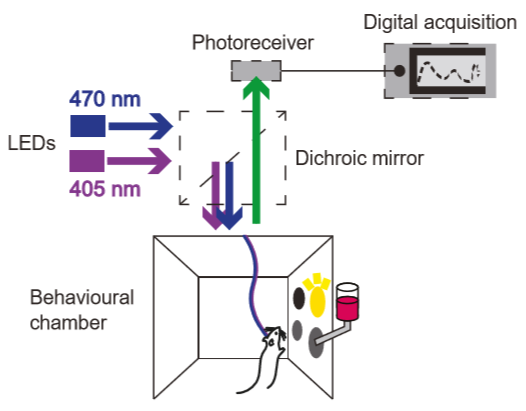
\includegraphics[scale=.50]{fiberphotometry.png} 
	\end{center} 
	\caption{\textit{Fiberphotometry experimental setup}}
	
\end{figure}

In the previous section, it has been shown a calcium imaging technique based on single neuron traces measured with single photon miniscopes. In this section, another common technique for calcium imaging will be presented: \textbf{fiberphotometry}. \\
The main goal of this technique is the same as the Inscopix imaging one, however technical equipment, methodology and results present substantial differences.\\
Relying on genetically encoded calcium indicators such as GCaMP, with fiberphotometry the fluorescence signal is recorded through \textit{optic fibers}, typically of length $300-400 \mu m$. An excitation of GCaMP is performed using a blu LED light at the appropriate wavelength ($470 nm$), which is transmitted through the optical cannula implanted in the mouse, while an emission green light ($525 nm$) is relayed to a photoreceiver. Often, a second excitation light (violet, $405 nm$), is used as well, to take into account autofluorescence and produce an isosbestic control signal [TESI PHD GIULIA].\\
 Finally, a software manages the output signal in order to perform filtering and give out a collective raw signal, separating the two contributions from blu and violet lights. Such signal, in contrast with the miniscope neuronal imaging, can only be an \textit{aggregate} signal of the observed area. This implies that the fiberphotometry technique produces signals at lower spatial resolution than the previously introduced technique. However, this technique is becoming always more used because the smaller accuracy is compensated by several positive factors:

\begin{itemize}
	
	\item The overall experimental setup for fiberphotometry results cheaper than the one for miniscope imaging 
	
	\item The procedure operated in mice are less invasive, and the subjects are more suitable to long freely behaving experiments
	
	\item The implant of the cannula is relatively easy to perform, and a good signal is collected even with fiber placements in the neighborhood of GECI -expressing populations [Siciliano and Tie 2018]
	
	\item Multiple areas of the brain can be investigated at the same time 
	
	\item Fiberphotometry can be used for other fluorescent indicators, such as norepinephrine (Feng et al., 2019), GABA (Marvin et al., 2019), glutamate (Liang et al., 2015),
	acetylcholine (Jing et al., 2018) and dopamine (Patriarchi et al., 2018)
	
	
	
\end{itemize}


\subsection{Synchronization of neural activities}

\begin{figure}[H]
	\begin{minipage}{\linewidth}
		\centering
		\begin{minipage}{0.6\linewidth}
			\begin{figure}[H]
				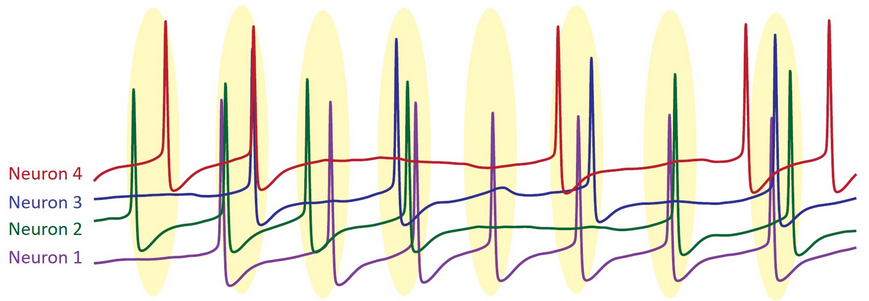
\includegraphics[width=\linewidth]{synch.png}
				
			\end{figure}
		\end{minipage}
		\hspace{0.05\linewidth}
		\begin{minipage}{0.6\linewidth}
			\begin{figure}[H]
				\includegraphics[width=\linewidth]{Intebrain.png}
				
			\end{figure}
		\end{minipage}
		
	\end{minipage}
\caption{\textit{Top: single neurons synchronization \\
		Bottom: overall activity synchronization}}
\end{figure}

In the previous sections, the concept of \textit{neural activity} has been introduced in its different shapes. Not only it can be identified with the electrical activity as well as the calcium one, but the activity necessarily refers to a specific area: it can be the activity of a single neuron or of a group of neurons in a ROI (often, in this case, the activity is attributed to the whole animal for that specific context); however, in any case, when talking about neural activity, the main object of interest is a \textbf{signal evolving in time}.\\
While historically the study of neural activity has mostly been the study of the behaviour of signals treated one by one, the focus, in the most recent years, is comprehending as well a more complex topic: the \textbf{synchronization between different activities}. The definition of synchronization between signals, not unique and assuming different shapes for different needs (chapter 2), can involve two types of correlations:

\begin{itemize}
	
	\item \textbf{Intraneuronal synchronization}: the signals of  single neurons show a correlated activity. Often (but not necessarily), the relevance of this phenomen is to look for correlations \textit{between} the same region of interest (ROI), namely for correlations between the neurons of the same animal in a particular area of its brain. However, the correlation could be investigated as well between different areas of the same individual, such as between neurons of different mice
	
	\item \textbf{Interbrain synchronization}: defining the activity of one individual (for example through a mean of its neuronal activities), one can study the synchronization between two individuals investigating correlations between their overall signals
	
\end{itemize}

The first type of synchronization, i.e. the correlation between a subset of neurons in the same individual, is a property of a neural circuit: it has been observed that the chain of firing of neurons (both in electrophysiology and calcium sense) often presents some \textbf{patterns}, in the sense that some neurons tend to show simultaneous peaks through times, or a similar order and timing of firing. The presence of correlated activity in a ROI has been shown to be linked with expressed behaviours [Frost et al. 2020], leading to the conclusion that \textbf{different behaviors can cause the synchronizations of different  subpopulations of neurons}.\\
This phenomenon could be independent by a rise of neural activity as consequence of an observed behaviour, in the sense that, in principle, it may happen that a rise in a correlated activity does not correspond to a rise in neural activity and viceversa. One of the goals of the correlation analysis is the \textbf{identification of a group of neurons encoding a specific behaviour}. The neuronal ensemble in the sense of synchronization may be different from the neuronal ensemble in the sense of activity peaks (even if often the intersection of the two is quite significant [Scheggia-Managò]).\\
In the second type of synchronization, the \textbf{interbrain synchronization}, the correlation analysis is performed between signals of different individuals; this could be intended both for single neurons and for  overall individual activities. Therefore, this type of synchronization is studied through an \textit{interaction} between two subjects. Again, the goal is either to find an ensemble of neurons which tend to correlate to the partner ones, either to show that in specific situations the correlations between subjects increases or decreases.\\

\begin{figure}[H]
	\begin{center}
		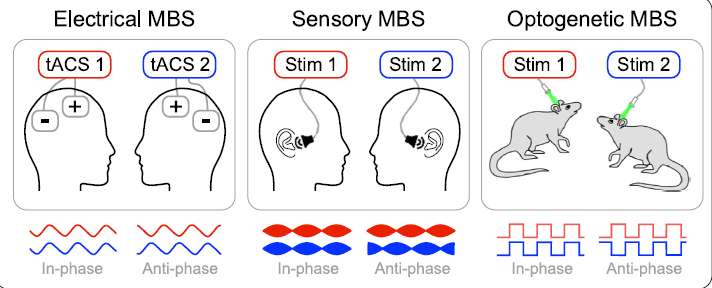
\includegraphics[scale=.70]{novembre.png} 
	\end{center} 
	\caption{\textit{Example of multi brain stimulation techniques}}
	
\end{figure}
Previous works ([Wass et al. 2020]) have been performed on humans in order to investigate the causes and effects of interbrain synchrony (often referred to as \textit{hyperscanning}). Performing an \textbf{electroencephalography (EEG)} on two interacting subjects, a strong connection has been identified between a rise in synchronization  and aspects like interpersonal coordination, cooperation and communication. In [Novembre et al. 2021], this relationship is further inspected: the simultaneous presence of synchronization and behaviour is not enough to establish a \textit{causality} between the two, which, instead, can be shown only by studying the effects which the manipulation of the first causes on the second, or viceversa. This is achieved through \textbf{multi brain stimulation (MBS)}: stimulation processes (usually of non invasive type in humans, invasive on animals) are performed on the subjects, and the provoked effects measured. Therefore, a correct analysis should combine the two approaches (hyperscanning and MBS) to be able to show true causality between interbrain synchrony and behaviour.
\\

As for interbrain analysis on mice based on microendoscopic calcium imaging, few works have been done and the topic is still ongoing. In one of the most significant papers, [Kingsbury et al. 2019], intracellular calcium has been recorded from neurons of the mPFC in two subjects interacting in an open arena.  The mean activity (as $\frac{\Delta F }{F}$ ) has been computed for every mouse, and the correlation between the two correspondent signals has been computed as well (using mostly cross-correlation, see chapter 2). The first result was that animals engaged in social interaction showed higher interbrain synchronization, reporting higher values of correlation during social interaction rather than solitary periods. Moreover, the abolishment of physical interaction, using a barrier, provoked as well an abolishment of interbrain correlation, meaning that the synchronization is not due to environmental factors, but instead strictly related to the direct interaction between conspecifics.\\

\begin{figure}[H]
	\begin{center}
		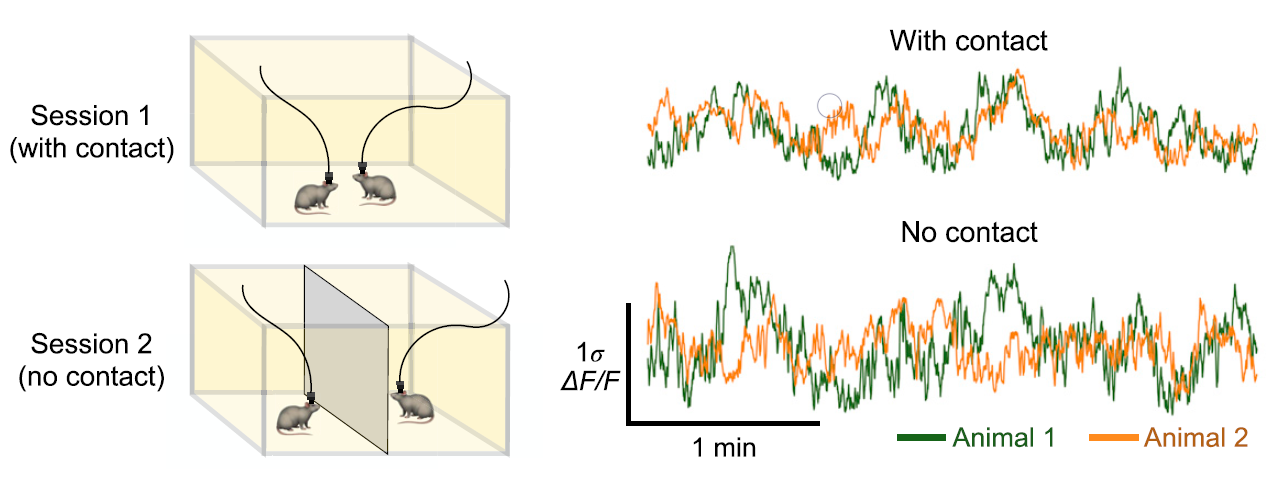
\includegraphics[scale=.70]{kingsbury.png} 
	\end{center} 
	\caption{\textit{Comparison of neuronal activities in the two mice with and without contact}}
	
\end{figure}


The second task performed in the experiment was the \textit{tube test}, in which the two subjects were placed facing each other in a horizontal tube, allowing the passage of only one individual. In this configuration, the mice can assume three types of behaviors: \textit{approach, push}, and \textit{retreat}; here animals showed again synchronization during the competitive encounters. In particular, a classification of neurons as behavioral cells allowed to link subgroups of neurons with the three types of behaviors depending on their activity values. Interestingly, the removal of these behaviour cells provoked a marked reduction of the correlated activity. Finally, between the two animals, it was evident that one would tend to assume the role of \textit{dominant} (prevalence of push behaviour), while the other of \textit{subordinate} (prevalence of retreat). Through generalized linear models (GLMs), it has been proposed a description of the dependence between the behaviour of one mouse and the neural activity of the other, observing that cells in subordinates responded more to the ones of the dominant than vice-versa. The consequence at synchronization level is that the opponent dictates the \textit{rhythm} for the subordinate's signal, making it able to predict the expected behaviour of one mouse based on the activity of the other.







\begin{figure}[H]
	\begin{minipage}{\linewidth}
		\centering
		\begin{minipage}{0.4\linewidth}
			\begin{figure}[H]
				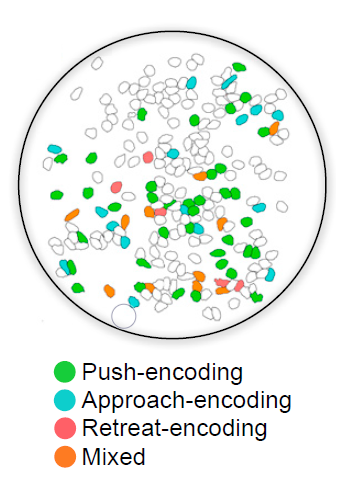
\includegraphics[width=\linewidth]{kingsbury2.png}
				
			\end{figure}
		\end{minipage}
		\hspace{0.05\linewidth}
		\begin{minipage}{0.5\linewidth}
			\begin{figure}[H]
				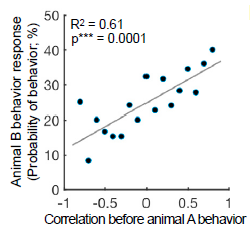
\includegraphics[width=\linewidth]{kingsbury3.png}
				
			\end{figure}
		\end{minipage}
		
	\end{minipage}
	\caption{\textit{Left: identification of behavioural neurons in the ROI \\
			Right: correlation between the interbrain synchornization preceding behaviour in one animal and the response probability of the interacting partner}}
\end{figure}

\newpage

\section{Interbrain data analysis}



\end{document}




\section{Introduction}

\begin{figure}[H]
\begin{center}
	\includegraphics[scale=.40]{ad_stab.png} 
\end{center} 
\caption{\textit{Numerical solution (blu) and real solution (black) in the  stabilized case for advection-diffusion problem}}

\end{figure}